\cleardoublepage

\section{曲线重建}

曲线重建主要分为两个部分,一个是连续化,即将离散的数据连续化;
另一部分是重建,根据连续的数据得到绝对坐标系下的曲线各点坐标。
根据传感器的种类不同,所测得的数据类型不同,这两步工作的执行顺序也可以不同。

如MEMS惯性传感器主要测量加速度数据,并对加速度数据进行二次积分而得到测量点位移,
故可以在计算测量点坐标之后再进行连续化;而像FBG传感器所得到的是测量点的曲率数据,
难以直接计算获得该点坐标,必须先对曲率数据进行连续化,然后再计算得出各点的坐标。

本文主采用更高精度、基于曲率数据的曲线重建方案。故可选用FBG传感器并假定可测得数据为两个正交方向的曲率。

\subsection{连续化}
图形学上常用的连续化算法(曲线)有贝塞尔(Bezier)曲线、B样条曲线、Catmull Rom样条曲线等;
而统计学上常用线性插值、多项式插值等。图形学连续化的常见目的是得到光滑曲线,而统计学则追求最小偏差。
由于“曲率光滑程度对曲线重建结果的影响”尚无理论研究,也超出了本文的研究范围,故本文采用其中最简便的线性插值法。

\subsection{重建}
常用的重建算法有基于Cartesian坐标系的拟合算法和基于Frenet坐标系的拟合算法。
其中Cartesian坐标系下的拟合算法拥有更高精度,而Frenet坐标系下的拟合算法更易于编程计算。
本文采用Cartesian坐标系。

\subsubsection{二维曲线}

\begin{center}
    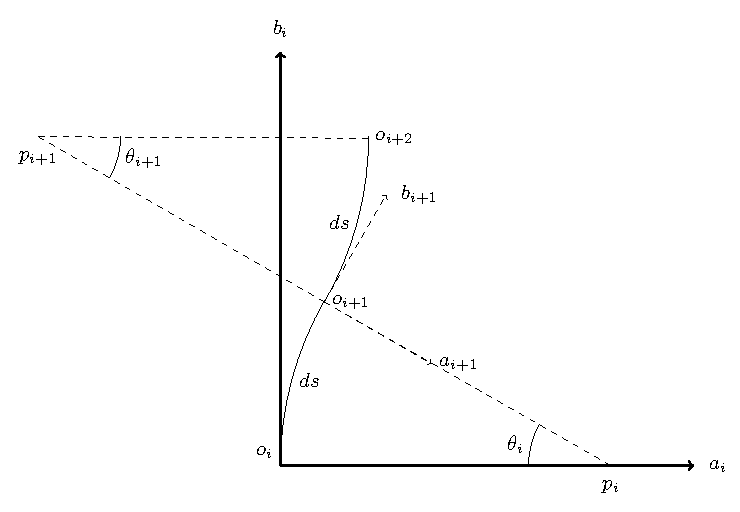
\includepdf[
        pages=1,
        scale=0.7,
        pagecommand={\pagestyle{fancy}},
    ]{2d-reconst.pdf}
\end{center}

如图所示,以曲线的每个$ds$微段的端点$o_i$为原点建立运动坐标系 $o_i-a_ib_i$,其中$b_i$是曲线在$o_i$点的切向量,$a_i$是法向量。

已知微段曲率值为$k_i$,则有:
\begin{equation}
\theta_i = ds\cdot k_i
\end{equation}
根据几何关系易得:

- 运动坐标系$o_i-a_ib_i$到运动坐标系$o_{i+1}-a_{i+1}b_{i+1}$的旋转矩阵$r_{i, i+1}$满足:
    \begin{equation}
    r_{i, i+1} = \left[
      \begin{matrix}
      cos \theta_i & sin \theta_i\\
      -sin \theta_i & cos \theta_i\\
      \end{matrix}
    \right]
    \end{equation}
    
- $o_{i+1}$在运动坐标系$o_i-a_ib_i$中的相对坐标$t_{i+1}$满足:
    \begin{equation}
    t_{i+1} = \frac{1}{k_i} \cdot \left[
      \begin{matrix}
    	1 - cos\theta_i\\
      sin\theta_i\\
      \end{matrix}
    \right]
    \end{equation}
    

故可得:

- 绝对坐标系$o_0-a_0b_0$到运动坐标系$o_i-a_ib_i$的旋转矩阵$R_i$满足:
    \begin{equation}
    R_i = \prod_{k = 0}^{i-1} r_{k, k+1}
    \end{equation}

- $o_i$ 到$o_{i+1}$在绝对坐标系中的位移向量$\vec{t_{i+1}}$满足
    \begin{equation}
    \vec{t_{i+1}} = Ri^{-1}\cdot t_{i+1}
    \end{equation}
    
- $o_i$在绝对坐标系中的坐标 $T_i$满足:
    \begin{equation}
    T_i = \left[
    		\begin{matrix}
        0\\
        0\\
      	\end{matrix}
      \right]
      + \Sigma_{k=1} ^ {i} \vec{t_i}
    \end{equation}
    
至此,我们通过二维曲线上各微段弧长和曲率拟合出了各端点的绝对坐标。

\subsubsection{三维曲线}

\begin{center}
    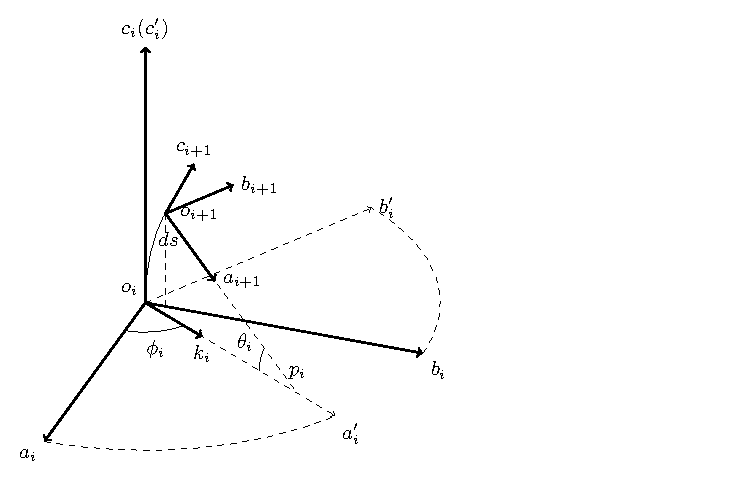
\includepdf[
        pages=1,
        scale=0.7,
        pagecommand={\pagestyle{fancy}},
    ]{coordinate-reconst.pdf}
\end{center}


在三维情况下,我们以曲线的每个$ds$微段的端点$o_i$为原点建立运动坐标系 $o_i-a_ib_ic_i$,其中$c_i$是曲线在$o_i$点的切向量,$a_i$是法向量,$b_i$是副法向量。
\begin{equation}
b_i = a_i \times c_i
\end{equation}
假设微段合曲率向量为$k_i$,则同样有:
\begin{equation}
\theta_i = ds\cdot |k_i|
\end{equation}
要求运动坐标系$o_i-a_ib_ic_i$到运动坐标系$o_{i+1}-a_{i+1}b_{i+1}c_{i+1}$的旋转矩阵$r_{i, i+1}$,需先求$k_i$与$a_i$的夹角$\phi_i$。

已知两个曲率分量$kx$和$ky$,将各运动坐标轴的$o-ab$平面叠加可得到下图的$o-xy$平面,其中$x$和$y$分别是两个曲率方向。由于$a$是曲线法向量,故$a_{i+1}$与$k_i$同向,即$a_{i+1}$与$a_{i+2}$的夹角$\phi_{i+1}$是合曲率向量$k_i$与$k_{i+1}$的夹角。

\begin{center}
    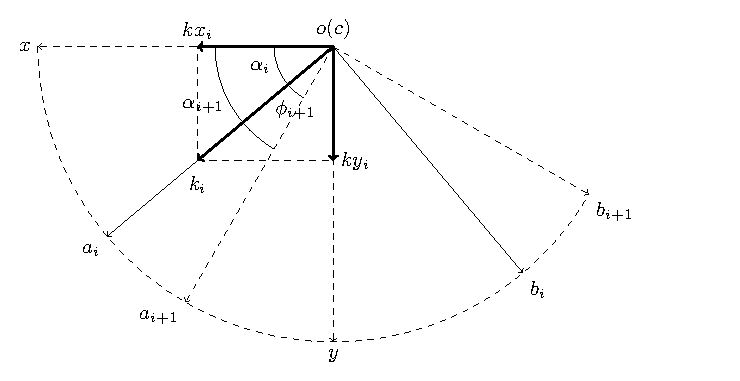
\includepdf[
        pages=1,
        scale=0.7,
        pagecommand={\pagestyle{fancy}},
    ]{iterate-phi.pdf}
\end{center}

又由于$x$的方向恒定(不发生扭转的情况下),故有:

\begin{align}
\phi_{i+1} &= \alpha_{i+1} - \alpha_i \\
\alpha_i &= arccos\frac{|kx_i|}{|k_i|} \\
k_i &= kx_i + ky_i \\
|k_i| &= \sqrt{(kx_i)^2 + (ky_i)^2}
\end{align}

算得$\phi_i$后可易得:

- 运动坐标系$o_i-a_ib_ic_i$到临时坐标系$o_i'-a_i'b_i'c_i'$的旋转矩阵$r_i'$满足:
    \begin{equation}
    r_i' = \left[
            \begin{matrix}
            cos\phi_i & -sin\phi_i & 0\\
            sin\phi_i & cos\phi_i & 0\\
            0 & 0 & 1\\
            \end{matrix}
        \right]
    \end{equation}
    
- 点$o_{i+1}$在临时坐标系$o_i'-a_i'b_i'c_i'$下的相对坐标$o_{i+1}'$满足:
    \begin{equation}
    o_{i+1}' = \frac{1}{|k_i|} \cdot \left[
      \begin{matrix}
    	1 - cos\theta_i\\
    	0 \\
      sin\theta_i\\
      \end{matrix}
    \right]
    \end{equation}
    
- 临时坐标系$o_i'-a_i'b_i'c_i'$到运动坐标系$o_{i+1}-a_{i+1}b_{i+1}c_{i+1}$的旋转矩阵$r_{i, i+1}$满足:
    \begin{equation}
    r_{i, i+1} = \left[
      \begin{matrix}
      cos \theta_i & 0 & -sin \theta_i\\
      0 &1 & 0\\
      sin \theta_i & 0 & cos \theta_i\\
      \end{matrix}
    \right]
    \end{equation}

故可得:

- 绝对坐标系$o_0-a_0b_0c_0$到临时坐标系$o_i'-a_i'b_i'c_i'$的旋转矩阵$R_i'$满足:
    \begin{equation}
    R_i' = r_i' \cdot \prod_{k = 0}^{i-1} r_k' \cdot r_{k, k+1}
    \end{equation}
    
- $o_i$ 到$o_{i+1}$在绝对坐标系中的位移向量$t_{i+1}$满足:
    \begin{equation}
    \vec{t_i} = Ri'^{-1}\cdot o_{i+1}'
    \end{equation}

- 绝对坐标原点$o_0$ 到$o_i$的位移向量$\vec{T_i}$满足:
    \begin{equation}
    \vec{T_i} = \Sigma_{k=1} ^ {i} \vec{t_i}
    \end{equation}

即$o_i$在绝对坐标系中的坐标 $T_i$满足:
\begin{equation}
T_i = \left[
    \begin{matrix}
    0\\
    0\\
    0\\
  	\end{matrix}
  \right]
  + \Sigma_{k=1} ^ {i} \vec{t_i}
\end{equation}


\subsubsection{核心算法实现}
\begin{lstlisting}[language=Rust, style=boxed]
pub fn reconstruct(&self, mut ai: Vector3<f64>, mut ri: Matrix3<f64>) -> Result<Vec<Point>, &'static str> {
    let mut points = Vec::with_capacity(self.splines.len()); // define points vector and reserve capacity
    let mut alpha_last = 0.;
    for (ka, kb) in self.splines.iter().cloned() {
        if ka == 0. && kb == 0. {
            // ka == kb == 0, no rotation, only translation.

            // Ti vector, a translation vector.
            let ti = ri.pseudo_inverse(0.000000001)? * Vector3::new(0., 0., self.ds);

            // ai + ti, to get absolute coordinate of current point
            ai += ti;
            let slice = ai.column(0);
            // push absolute coordinate of current point
            // println!("(x, y, z): ({}, {}, {})", slice[0], slice[1], slice[2]);
            points.push(Point {
                x: slice[0] as f32,
                y: slice[1] as f32,
                z: slice[2] as f32,
            });
        } else {
            let k = (ka.powi(2) + kb.powi(2)).sqrt(); // composite curvature
            let theta = k * self.ds;
            let alpha = (ka / k).acos();
            let phi = alpha - alpha_last;
            alpha_last = alpha;

            let cos_phi = phi.cos();
            let sin_phi = phi.sin();
            let cos_theta = theta.cos();
            let sin_theta = theta.sin();


            ri = Matrix3::new(
                cos_phi, -sin_phi, 0.,
                sin_phi, cos_phi, 0.,
                0., 0., 1.,
            ) * ri;

            // get generalized inverse of ri; then dot product relative coordinate
            let ti = ri.pseudo_inverse(0.000000001)? * Vector3::new((1. - cos_theta) / k, 0., sin_theta / k);
            ai += ti;
            let slice = ai.column(0);
            // push absolute coordinate of current point
            // println!("(x, y, z): ({}, {}, {})", slice[0], slice[1], slice[2]);
            points.push(Point {
                x: slice[0] as f32,
                y: slice[1] as f32,
                z: slice[2] as f32,
            });

            ri = Matrix3::new(
                cos_theta, 0., sin_theta,
                0., 1., 0.,
                -sin_theta, 0., cos_theta,
            ) * ri;
        }
    }
    Ok(points)
}
\end{lstlisting}

\subsection{重建效果与误差分析}

本小结主要内容是重建算法的效果展示与误差传递分析。
为了便于画图与分析,所用曲线为二维标准余弦曲线。

\subsubsection{结果与误差}

\begin{center}
    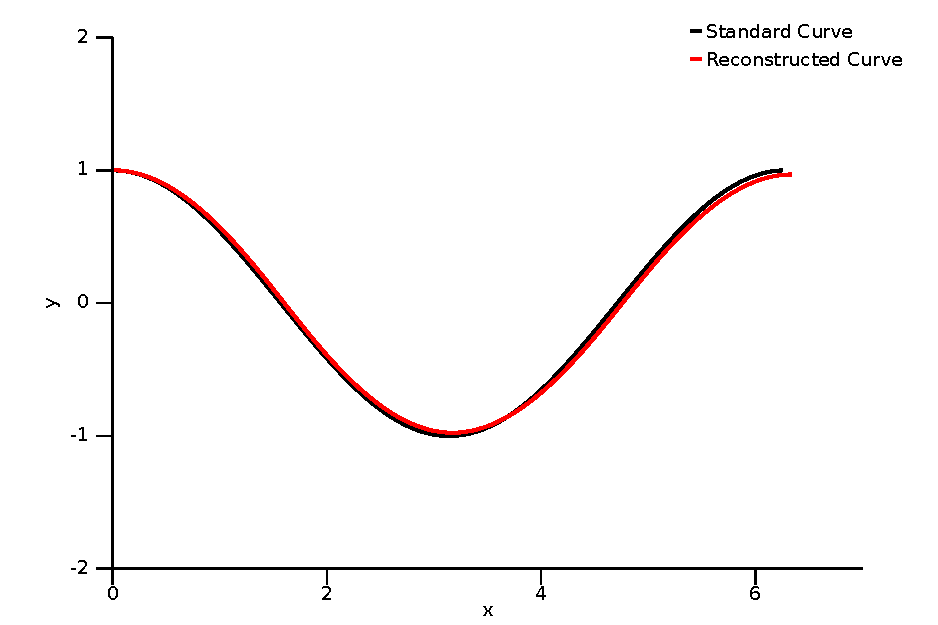
\includepdf[
        pages=1,
        scale=0.7,
        pagecommand={\pagestyle{fancy}},
    ]{cos.pdf}
\end{center}

\begin{center}
    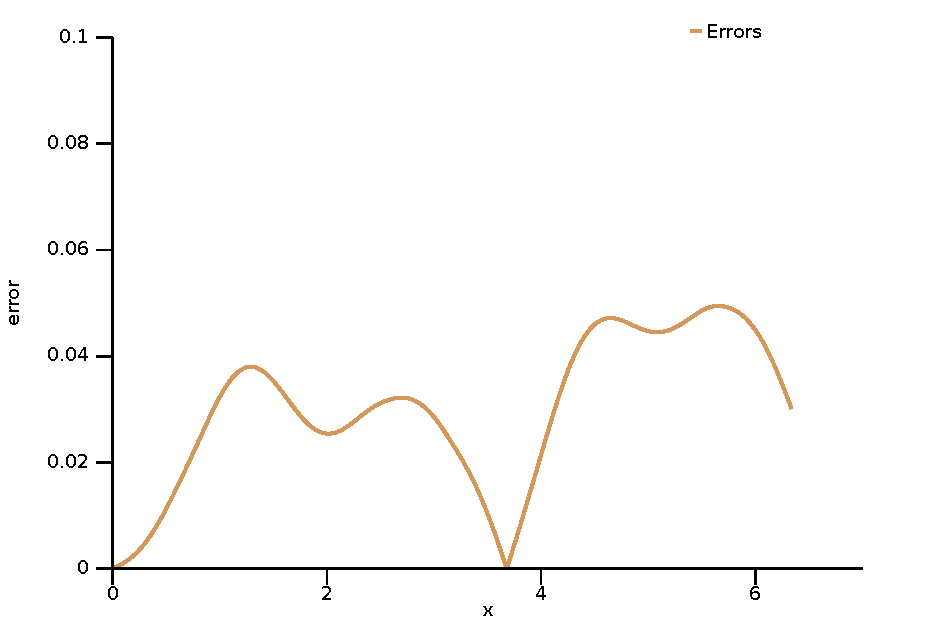
\includepdf[
        pages=1,
        scale=0.7,
        pagecommand={\pagestyle{fancy}},
    ]{cos-error.pdf}
\end{center}

\subsubsection{不同步长下的误差}

\begin{center}
    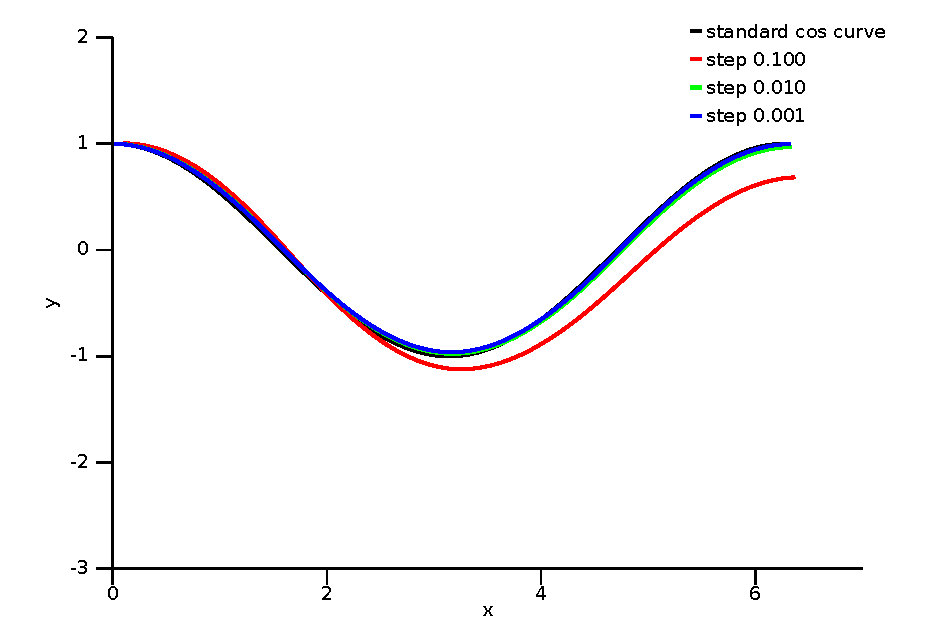
\includepdf[
        pages=1,
        scale=0.7,
        pagecommand={\pagestyle{fancy}},
    ]{cos-diff-step.pdf}
\end{center}

\subsubsection{误差传递}

\begin{center}
    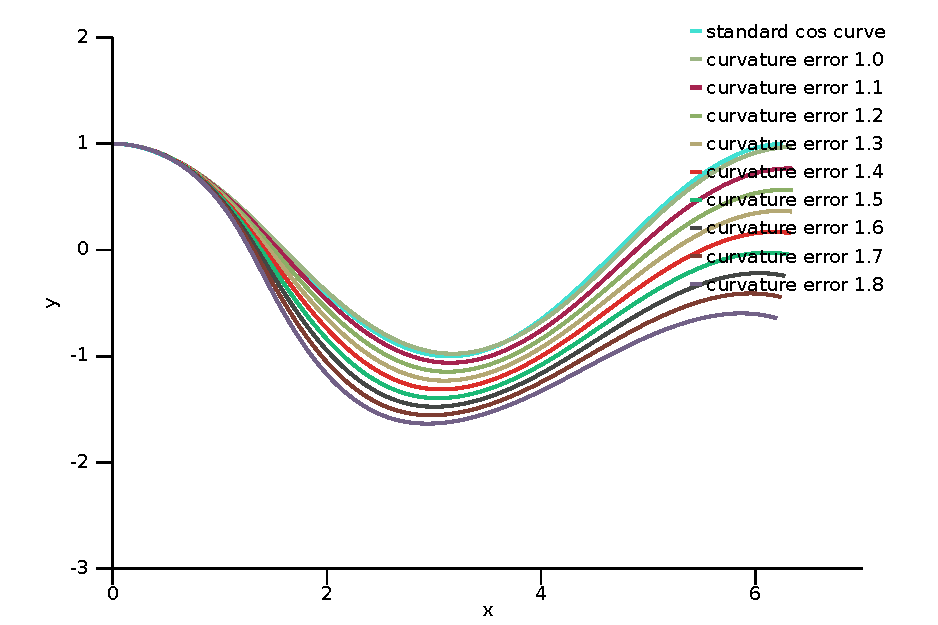
\includepdf[
        pages=1,
        scale=0.7,
        pagecommand={\pagestyle{fancy}},
    ]{cos-single-error.pdf}
\end{center}

\begin{center}
    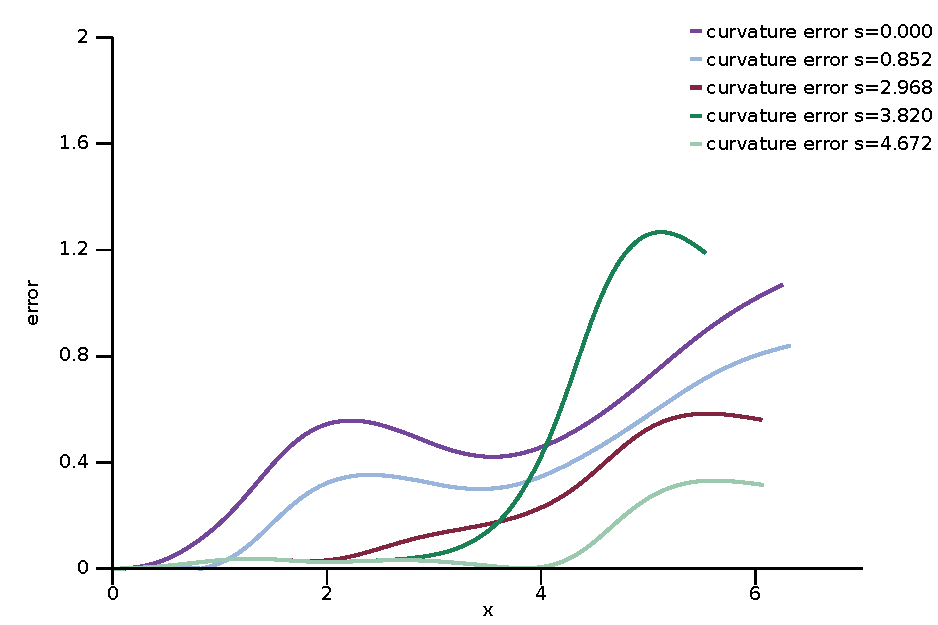
\includepdf[
        pages=1,
        scale=0.7,
        pagecommand={\pagestyle{fancy}},
    ]{cos-multiple-error.pdf}
\end{center}
